\section{Moteur de jeux combinatoires abstrait}


% présenter les principaux algorithmes utilisés comme moteur de jeu combinatoires absrtaits
%methode de monte carlo
%min max


% evaluer la complexité théorique en temps des algorithmes présentés.

Implémenter un algorithme pour jouer à des jeux combinatoires contre ordinateur est l'un des objectifs principaux du projet
Hex-Ta(c)tique mais une problématique importante apparait: quels sont les algorithmes qui permettent à un ordinateur
de jouer à un jeu combinatoire abstrait ? Quels sont leurs points forts et faibles ? Dans cette section nous allons
présenter 2 algorithmes principaux qui aident à répondre à ces questions: la recherche arborescente \emph{Monte-Carlo} (Monte carlo Three Search) 
et l'algorithme du \emph{min-max} avec élagage alpha beta:

\subsection{La recherche arborescente Monte-Carlo}

\paragraph{Présentation}
La recherche arborescente Monte Carlo ou Monte Carlo tree search (MCTS) est un algorithme de recherche heuristique.
Il est principalement utilisé dans le cadre de mise en place d'intelligence artificielle pour des jeux tels que le go mais pas uniquement.
En effet il est aussi utilisé pour les moteurs de jeux des échecs comme le moteur Alpha Zero de Google qui est
l'un des leaders en terme d'intelligence de jeux aux échecs. Cet algorithme peut même être implémenté dans des jeux où le hasard 
apparait par exemple au poker.

\paragraph{MCTS - fonctionnement succinct}
Monte Carlo Tree Seach ou MCTS est un algorithme qui explore l'arbre des possibles. La racine est la configuration initiale du jeu.
Chaque nœud est une configuration (une situation en jeu) et ses enfants sont les configurations suivantes. MCTS conserve en mémoire 
un arbre qui correspond aux nœuds déjà explorés. Une feuille de cet arbre est soit une configuration finale (donc un des joueur a gagné)
soit un nœud dont aucun enfant n'a encore été exploré. Dans chaque nœud, on stocke deux nombres : le nombre de simulations gagnantes, 
et le nombre total de simulations. 

A chaque itération MCTS va chercher la feuille la plus prometteuse, comprendre la suite de coups qui possède la meilleure heuristique, 
et ensuite depuis cette feuille créer, grâce aux règles du jeu, une nouvelle feuille au hasard dans le but d'atteindre une configuration finale.
Dans le cas où on trouve une configuration gagnante pour un joueur, on va incrémenter le nombre de simulations gagnantes, pour les nœuds
correspondant au joueur, dans les parents de la feuille que l'on vient de créer.
L'algorithme répète cette opération un certain nombre de fois avant de choisir un coup, ie: choisir le coup qui a le plus de simulations
gagnantes et le moins de simulations totales.

%exemple.\dots


\subsection{MinMax}

\paragraph{Présentation}
L'algorithme MinMax, comme MCTS, est un algorithme décisionnel mais celui-ci s'applique sur des jeux à somme nulle: c'est-à-dire
un jeu où la somme des gains et des pertes de tous les joueurs est égale à 0. Cela signifie donc que le gain de l'un constitue 
obligatoirement une perte pour l'autre. L'algorithme va utiliser cette propriété dans sa recherche pour le meilleur coup possible.
En effet il amène l'ordinateur à passer en revue toutes les possibilités pour un nombre limité de coups et à leur assigner une valeur 
qui prend en compte les bénéfices pour le joueur et pour son adversaire. Le meilleur choix est alors celui qui minimise les pertes 
du joueur tout en supposant que l'adversaire cherche au contraire à les maximiser (d'où le nom MinMax).

\paragraph{MinMax - fonctionnement succinct}
Comme le MCTS le MinMax va explorer l'arbre des possibles. L'algorithme va explorer toutes les possibilités et mettre une valeur positive ou négative
à chaque feuille de l'arbre qui sont des nœuds terminaux ou des nœuds à la profondeur de recherche maximale.
Une valeur est positive si la position favorise le joueur que joue l'ordinateur (le joueur maximisant) et négative dans le cas contraire.
Les nœuds non feuilles héritent de leur valeur a l'aide de leurs enfants.
Ainsi, les nœuds conduisant à un résultat favorable, comme une victoire, pour le joueur maximisant ont des scores plus élevés que les nœuds 
plus favorables pour le joueur minimisant. Les valeurs heuristiques pour les nœuds feuilles terminaux (fin du jeu) sont des scores correspondant 
à la victoire, à la défaite ou à l'égalité pour le joueur maximisant. Pour les nœuds feuilles non terminaux à la profondeur maximale de recherche, 
une fonction d'évaluation estime une valeur heuristique pour le nœud. La qualité de cette estimation et la profondeur de recherche déterminent la 
qualité et la précision du résultat final de minimax.

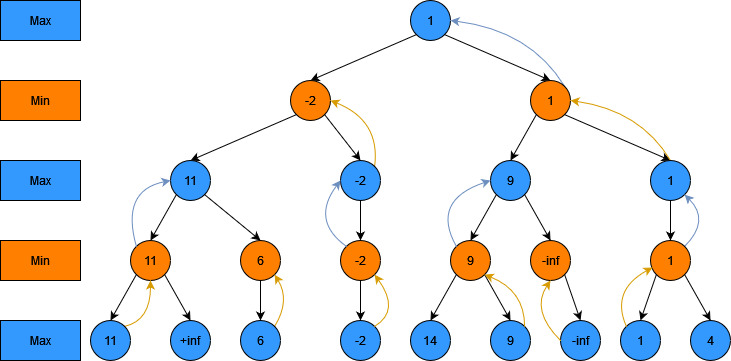
\includegraphics[width=0.4\textwidth]{root/MinMax.jpeg}